\setchapterpreamble[u]{\margintoc}
\chapter{Theoretical foundation}
\labch{theory}

Machine learning covers a set of problems and tools that overlaps several disciplines. As such, in order to tackle machine learning problems, it is necessary to lay some foundations which help grasp all the concepts involved. Even though this is a rapidly evolving field, there are fundamental topics that remain applicable.

The objective of this chapter is to provide the reader with the definitions, descriptions and examples that allow to understand the rest of this work. We will try to assume little-to-no prior knowledge about machine learning, thus making it as accessible as possible. The following sections go over the basic subjects of machine learning, build the core concepts of deep learning and arrive to the main tools that will be used along the rest of this book, autoencoders.

\section{Machine learning fundamentals}[ML fundamentals]

Machine learning\index{machine learning} differs from other kinds of computer science disciplines in that its objective is not to give precise instructions for the machine to follow, but instead to provide some form of experience that the machine must learn from in order to extract some information or display some behavior \sidecite{deisenroth2020mathematics}. The algorithms developed for machine learning are essentially mechanisms that take in a certain amount of data, process it and compute the necessary steps to fulfill a specific objetive related to the data. Their output is usually a model, that is, a representation of an approximate solution to the problem. 
 
\subsection{Data and models}

\begin{margintable}
\caption[An example dataset describing features of different kinds of animals.]{\label{tbl:dataset}An example dataset describing features of different kinds of animals. Each feature can be numerical (length, legs) or categorical (wings, species).}\footnotesize
\resizebox{\linewidth}{!}{\begin{tabular}{rrrl}\toprule
Length & Legs & Wings & Species\\\midrule
0.40 & 4 & No & Dog\\
0.01 & 6 & Yes & Fly\\
1.45 & 0 & No & Dolphin\\\bottomrule
\end{tabular}}
\end{margintable}

Datum (plural \textit{data})\index{data} usually refers to the minimal unit of machine-readable information, for example, the height of a person (numerical value), whether they are an adult or not (binary categorical value), their country of origin (categorical value) or their given name (character string).

A \textit{dataset}\index{dataset} is a collection of data, usually organized into a table. It contains several \textit{samples}\index{sample}, which correspond to each one of the cases of the problem from which the machine will be able to learn before being presented with new cases. \textit{Variables}\index{variable} are each one of the aspects that have been measured or that characterize each sample. They determine the type of data (character strings, numbers, dates) and the range where values are taken. A usual distinction of numerical variables is between continuous and discrete ones, the former corresponding to real intervals and the latter with a countable set of possible values. 

Samples are typically distributed in rows and variables in columns. \autoref{tbl:dataset} shows an example of dataset with 3 samples and 4 variables, where each variable corresponds to a specific kind of data: \textit{length} is a continuous numerical variable, \textit{legs} is discrete numerical, \textit{wings} is binary categorical and \textit{species} is categorical.

% \subsection{Models}

A \textit{model}\index{model} is an abstraction of a dataset that enables the machine to perform the desired operations, for example, generating new data similar to the available, or assigning a category to new data points. A good model should be faithful to the available data, incorporating enough information to describe its behavior and potential relations between variables, so that it can be used as a description of the data and as a tool for solving tasks related to it. Models typically follow some template which includes a range of parameters that can be adjusted in order for the resulting model to represent the data. We will call these templates \textit{untrained models}, whereas the final results will be \textit{trained models}.



\subsection{Learning and types of learning}

In the context of machines learning from data, several types of learning are usually distinguished, according to the feedback that the machine receives while processing data. This concept is known as \textit{supervision}, and usually relates to whether there are available solved cases for the specific problem at hand. A solved case is composed of an input instance and an associated solution or \textit{label}, which may be a numerical value, a categorical value or a more complex structure. Attending to the availability of labels for the learning algorithm, the following learning paradigms are considered \cite{bishop2006pattern}:
 
\begin{itemize}
    \item Supervised learning %(SL\nomenclature{SL}{Supervised learning})
    \item Unsupervised learning
    \item Semi-supervised learning
    \item Reinforcement learning
\end{itemize}

\subsubsection{Supervised learning}

In a supervised learning\index{supervised learning} setting \sidecite{Caruana2006AnEC}, every observed case of the problem in the dataset is coupled with its solution, so that the machine can learn a mapping out of those associations, from the space of the instances (input space) to the one of the labels (output space). Models generated by learning algorithms in this contexts are usually known as \textit{predictors}, since for each new data point they must guess a label in the output space. For example, in \autoref{tbl:dataset}, an appropriate objective task for a supervised learning algorithm is to predict the species of an animal, knowing the rest of its characteristics. 

Common supervised learning problems are \textit{classification} and \textit{regression}. They differ in the type of output that the predictor must produce: classification implies that the output space is finite, thus the label is just one of a certain number of available \textit{classes}, whereas regression involves guessing a real value from a continuous interval. 

\subsubsection{Unsupervised learning}

The scenario of unsupervised learning\index{unsupervised learning} \sidecite{celebi2016unsupervised} covers problems where the solution is not known for the data that is available and, as a result, the model cannot be provided with supervision. Instead, the user of an unsupervised learning algorithm looks to find some sort of inner structure or hidden patterns in the data.

One case where unsupervised learning methods are convenient is when trying to find the most useful variables in a dataset, or even transform the original features onto a more compact set of variables which prevent redundancy and maximize efficiency in relation to information provided per feature. Another typical task is finding associations between items present in the data points, like related articles in a shopping bag or recommended moviess. 

\subsubsection{Combinations of supervised and unsupervised learning}

There are special cases where the task that is being approached is not entirely supervised but not completely unsupervised either, but a mix of both.

The most common combination emerges when the presence of labels in the observed data is mixed, that is, there are instances with associated labels and others with missing labels. This learning paradigm, known as \textit{semi-supervised learning}\index{semi-supervised learning} \sidecite{van2020survey}, is of interest in many real-world problems, since annotating each one of the collected data instances with its corresponding label can be costly and time-consuming~\sidecite{vanEngelen2019ASO}. 

Another relevant area that combines predictive and descriptive learning is that of \textit{subgroup discovery}\index{subgroup discovery} \sidecite{Herrera2010AnOO}, a task where the objective is to find unusual relations (rules) between the input variables and the target variable. Instead of learning to predict this variable, the idea is to identify interesting subsets of instances according to their relation to the target variable and the rest of samples.

\subsubsection{Reinforcement learning}\index{reinforcement learning}

A different strategy for machines to learn consists in providing them with positive or negative reinforcements according to their behavior \sidecite{kaelbling1996reinforcement}. Instead of providing the algorithm with the complete solution for each problem instance, usually a score is given, evaluating the current solution against some criteria. This learning paradigm fits well with problems where multiple solutions can be acceptable, so the actual solving process is not as important as obtaining the desired result, as well as situations where the aim is to find the most efficient solution. Notable examples of this kind of learning are tabletop games like AlphaGo for Go \sidecite{silver2016mastering} and even strategy videogames like AlphaStar for StarCraft II \sidecite{vinyals2019grandmaster}.

% \subsection{Traditional machine learning algorithms}

\section{Obstacles when learning models}

Machine learning models can come across several kinds of difficulties that are relevant to analyze since they are related to the tools and solutions studied in this thesis. Primarily, we will focus on improving the feature sets and tackling certain aspects of supervised learning problems.

\subsection{Feature sets}

The feature set, as explained in Chapter~\ref{ch:intro}, corresponds to the space where each sample takes values. The same events may be expressed by different feature sets according to the information collection procedures. For example, a spoken command may be represented by a precise sound file that was recorded or by the words that were uttered. In the former case, the feature set could be the presence of each frequency at each time point. In the latter, a possible set of features would indicate whether each word from a predefined list was present or not in the sentence.

Traditional algorithms for adjusting models tend to process data "as is", which means that they perform few transformations (or none) to each vector before using them directly to fit model parameters. This causes them to underperform when the representation of the vectors (i.e. the set of features) is not ideal. As a consequence, it is usually convenient to preprocess data beforehand, using one or several tools that will manipulate the features looking to improve the performance of the learning algorithm. This is known as \textit{feature extraction}, feature learning or representation learning \sidecite{bengio2013representation}. 

\subsection{Potential issues with supervised problems}

Although supervised learning tasks provide the desired answer for all observed cases, there are a wide variety of obstacles that can prevent a learning algorithm from finding an acceptable solution.

The structure of the task can itself be a hindrance. The scheme that most algorithms are designed to tackle is that of a binary classification problem. This is characterized by the categorization of instances in one of two possible classes, which can be represented as a binary variable which acts as the target. Each instance is in turn represented by a vector valued in a set of variables. Although this is the simplest setting for a supervised machine learning problem, and many methods are initially created with it in mind for this reason, real world situations usually need more complex approaches.

One possible case is problem objects being represented by several data points, either homogeneous or heterogeneous according to whether they come from the same feature space. For example, one molecule may present various forms \sidecite{dietterich1997solving}, where one of them may present a valid solution, rendering that molecule apt to solve the studied problem. This is known as a \textit{multi-instance} learning task, while a \textit{multi-view} one would have the data points belonging to different sources (and different feature spaces) \sidecite{sun2013survey}, like social media posts with associated image and text. Learning methods are typically applied with a one-to-one input-target association in mind, so these types of input structures become harder to work around.

Equivalently to each problem case being structured differently to a feature vector, the target can also become more complex. Many real world situations are better represented with more than one target variable. For example, tags in text documents can appear simultaneously, so predicting them will require a multilabel classification algorithm \sidecite{herrera2016multilabel}. A similar case applies to continuous values in targets, leading to multi-output regression methods \sidecite{borchani2015survey}.

Moreover, combinations of the previous nonstandard inputs and outputs structures can coexist, like in multi-instance multilabel problems \sidecite{zhou2012multi} or multi-view multilabel ones \sidecite{zhu2020global}.

% - small intro to nonstandard problems

Different issues can arise that make certain classes hard to learn by classifiers due to their size, location or lack of representation within the training set itself. This phenomenon is broadly known as data complexity\index{data complexity} \sidecite{ho2002complexity}, and in some cases as difficult classes \sidecite{galar2014empowering}, if the complications are related to a specific class. Data complexity can be caused by the feature set not fully being able to separate instances of different classes, class boundaries being highly nonlinear or composed of several disjoint subsets, or a class being notably underrepresented with respect to the rest, among other factors.

% - small intro to difficult classes

\section{Deep learning}

An alternative approach to extracting features before training a predictor 
is to embed the feature extraction stage within the untrained model itself, and learn the best features at the same time that the final model (a classifier, regressor, segmentor...) is trained. When this process is organized layer-wise, the overall model is called a \textit{deep learning} model \sidecite{goodfellow2016deep}\index{deep learning}.

Deep learning model design comprises two complementary elements: the type of \textit{layers} that build up the network and determine the type of data that can be processed, and the \textit{architecture} itself, that is, the way these layers are organized and allow to perform one task or another with the provided data. For example, one could build a classification network out of recurrent units for sentiment analysis, or an encoder-decoder network out of convolutional layers for image segmentation. The fundamental types of layers as well as the most relevant architectures are explained next.

\subsection{Neural networks according to layer operations}[Layer operations]\label{sec:layers}

Not every kind of neural network is prepared to deal with every type of dataset. Their main advantage is that they can become specialized in certain structures, such as sequential data (sound, speech, language), bidimensional data (images) and three-dimensional data (video). This specialization while preserving the same training strategies and essential implementation methods is what sets them apart from traditional learning methods, which are more fixed in their way of working through data.

\subsubsection{Dense networks}

Dense deep networks, also known as fully connected\index{fully connected} networks, are essentially the same as MLPs. Their main operation in each layer is matrix product, where a parameter matrix is used to extract the values of each layer out of those of the previous one. More formally, is $x$ is an input vector, $W$ is the parameter matrix and $b$ is a bias parameter, the dense layer performs the following computation:

\begin{equation}
    f(x)=Wx + b\quad W\in \mathcal M_{n\times m}(\mathbb R), x\in\mathbb R^m, b\in\mathbb R^n~.
\end{equation}

These networks are called fully connected because each value in the output is able to draw information from all values in the input vector. This is especially useful when variables are not structured since the order of variables  will not affect the training.

\subsubsection{Convolutional networks}

\begin{marginfigure}
    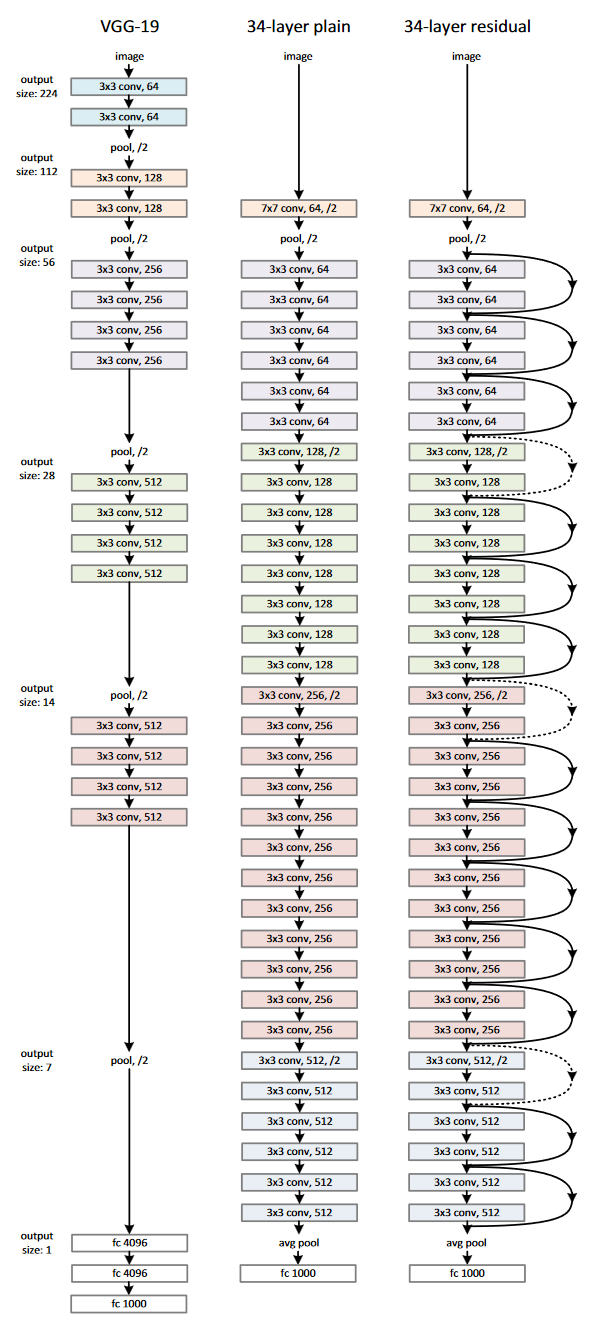
\includegraphics{resnet}
    \caption[Comparison of the architectures of several CNNs.]{\label{fig:resnet}Comparison of the architectures of several CNNs, from left to right: VGG-19, a CNN with 36 layers and a residual CNN with 36 layers. Figure from \cite{he2016deep}.}
\end{marginfigure}


Convolutional networks\index{convolutional network} (CNNs) emerge out of the need to adapt operations to bidimensional data, as well as reduce the computational complexity of dense networks when treating this type of high-dimensional data. Since the matrix used in a dense layer has $n\times m$ parameters, $m$ being the number of variables in the input vector and $n$ the number of variables in the output vector, the amount of floating point operations required to compute the result is $O\left(nm\right)$.

In a CNN, a certain number of matrices typically named \textit{channels} is computed out of the input matrix. Each one is composed of values calculated by convoluting the original matrix with a weight matrix, called \textit{kernel}, which is usually of a fixed small size: $3\times 3$ up to $9\times 9$. Each pixel $(i, j)$ in a filter resulting from convoluting a kernel $K$ over the input $I$ can be computed as follows:
\begin{equation}
    f(i,j)=\left(K\ast I\right)(i,j)=\sum_{m}\sum_{n}I(i-m,j-n)K(m,n)~.
\end{equation}
By keeping $k$, the size of the kernels, notably smaller than the input image, the complexity of convolution is $O(kn)$ and it requires much fewer parameters than matrix multiplication.  This makes CNNs appropriate for image-related tasks such as image classification, segmentation and object detection. They can also extend to tridimensional data such as video segments.


Most current neural network libraries implement cross correlation instead of the discrete convolution, which does not affect the results since equivalent kernels can be learned for it. The operation is still called convolution in most cases, and the only change is a sign flip for $m$ and $n$:
\begin{equation}
    f(i,j)=\left(I\ast K\right)(i,j)=\sum_{m}\sum_{n}I(i+m,j+n)K(m,n)~.
\end{equation}

Convolution is not the only stage performed by CNN. The other important step is \textit{pooling}\index{pooling}. This function outputs a smaller version of its input by summarizing nearby values. For example, max pooling \sidecite{zhou1988computation} takes the maximum out of a rectangle of the input matrix and outputs that as a single value, reducing in this way the size of the matrix.

Computer vision has been one of the fundamental applications of deep learning and CNNs have evolved greatly as a result, with many improvements and extensions such as residual connections (see Figure~\ref{fig:resnet}), breakdown of convolutions into smaller ones \sidecite{7780677}, and pruning strategies \sidecite{lin2019towards}.


\subsubsection{Recurrent networks}

{In a recurrent neural network (RNN)\index{recurrent network}, some parts of the computation of the network at each step, e.g. the output, are fed as input in the next one. This creates a ``memory'' which allows the RNN to remember previous outputs when making predictions. RNNs are used for tasks such as speech recognition and language translation, where the order of the input is important and past outputs are relevant for the next predictions.}

\begin{marginfigure}
    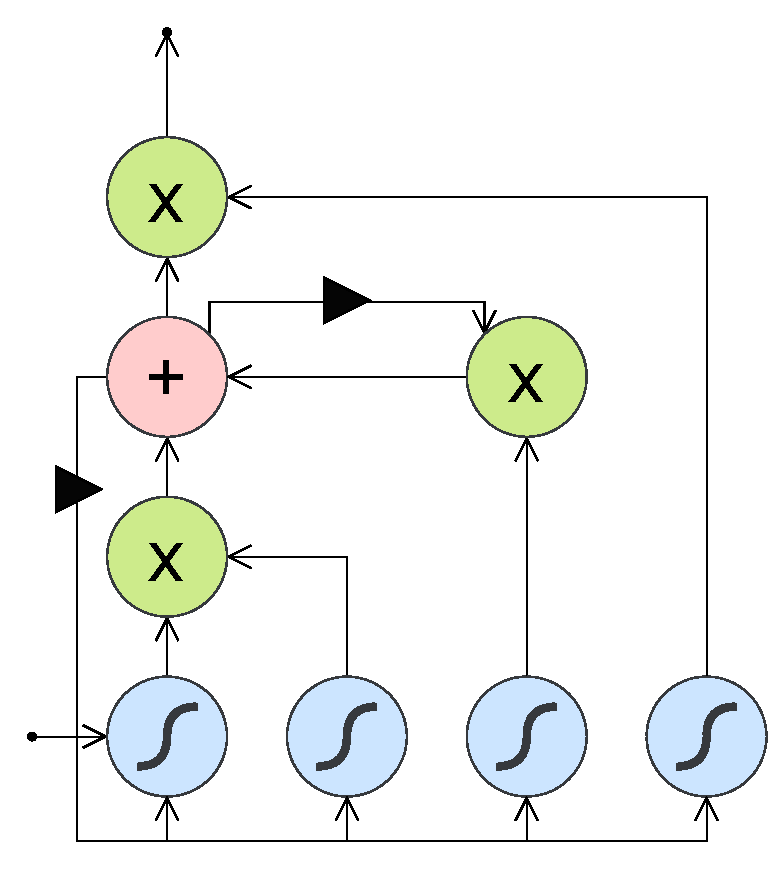
\includegraphics[width=\linewidth]{lstm}
    \caption[Diagram for an LSTM.]{\label{fig:lstm}Diagram for an LSTM where blue units are gates (sigmoidal or tanh activations), green units are products and pink units are sums. Triangles over data flows indicate values that are fed at the next step.}
\end{marginfigure}

A popular kind of RNN units are long short-term memory\index{long short-term memory} (LSTM) units \sidecite{hochreiter1997long}, which add a self-loop controlled (\textit{gated}) by another unit so that the memorized information can be eventually forgotten. See Figure~\ref{fig:lstm} for a detailed schematic of this type of unit.


\subsubsection{Attention and transformers}

Attention\index{attention} mechanisms started in encoder-decoder recurrent networks as a system to identify parts of speech that are more relevant than others within the input data while decoding is in process \sidecite{bahdanau2014neural,luong2015effective}. Instead of compacting all the inputs into an encoded vector and decoding from there, attention allows to have all information available and focus on just the important pieces at each decoding step. There exist several ways of applying attention according to the elements that interact with one another, including self-attention, local attention and global attention.

\begin{marginfigure}
    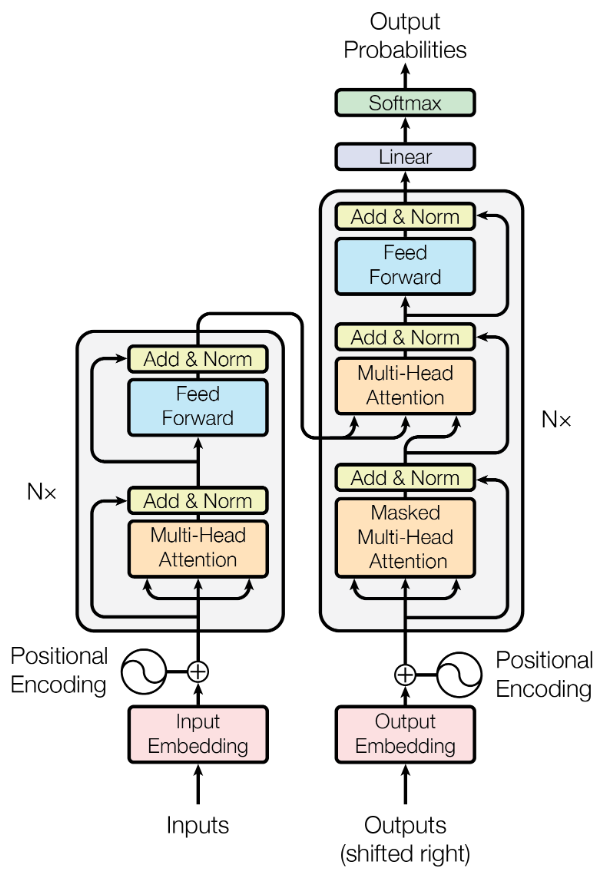
\includegraphics{transformer}
    \caption[Original architecture diagram of the Transformer.]{\label{fig:transformer}Original architecture diagram of the Transformer. Source: \cite{vaswani2017attention}.}
\end{marginfigure}

Based on the concept of attention, transformers\index{transformer} \sidecite{vaswani2017attention} were conceptualized by simply avoiding recurrent units and building the whole network around stacked self-attention operations. Figure~\ref{fig:transformer} shows how a transformer is organized. 
Transformers have been applied beyond machine translation to many other natural language tasks, where they are currently the state of the art \sidecite{devlin-etal-2019-bert}. Some proposals have tackled computer vision as well \sidecite{liu2021swin}, but are being matched in performance by attention-free models such as \sidecite{chen2021cyclemlp}.

\subsection{Network architectures}

Neural layers can be organized in different formations and connected in various ways in order to achieve specific solutions. The structure and connections of a network are known as its architecture\index{architecture}.

\subsubsection{Classifiers and regressors}

Classifiers and regressors are very common types of neural network architectures. The key to obtaining a label output from a network is to stack layers which transform and progressively reduce the dimension of the original data, up to the last layer where the class is selected or a numerical value is predicted. 

Some classification networks are trained and tested against well known benchmarks, becoming a reference for further works and even a basis for other tasks, leveraging the already extracted knowledge by means of \textit{transfer learning}\index{transfer learning}. For instance, the VGG-19 and ResNet networks shown in Figure~\ref{fig:resnet} are standard tools for general image classification.

\subsubsection{Encoder-decoder structures}

There exists a category of deep architectures composed of two components, an \textit{encoder}\index{encoder} and a \textit{decoder}\index{decoder}, where there is an interest in the model operating first with the features in order to obtain higher-level features (encoding) and then developing these features back onto more detailed and specific versions.

For example, when the objective task is to segment the pixels in an image, that is, label each pixel with one of several classes, a possible solution is to compute abstract, high-level features for the image, and use those to classify each pixel next \sidecite{minaee2021image}. This allows to analyze the neighborhoods of each pixel before assigning it to a class, which will probably lead to more cohesive segmentations. Using an encoder-decoder structure, the encoder would compute these low-resolution but high-level features, and the decoder would perform the detailed labeling task out of the extracted information.

Similarly, an encoder-decoder scheme made out of recurrent units, also known as a \textit{sequence-to-sequence} model \sidecite{prabhavalkar2017comparison}, could serve as basis for a language translation system. The encoder would extract an intermediate representation for the meaning of the original sentence and the decoder would transform that onto the target language.

A special subset of encoder-decoder architectures are autoencoders, which are further described next.

\subsubsection{Autoencoders}

\begin{marginfigure}
    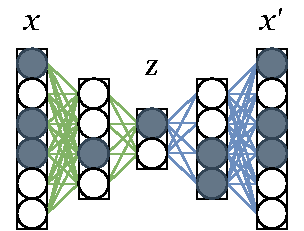
\includegraphics{basic-fc-ae}
    \caption{\label{fig:basicae}Schematic structure of a fully connected autoencoder.}
\end{marginfigure}

Essentially, an \textit{autoencoder}\index{autoencoder} is an encoder-decoder architecture which is trained to map its inputs onto its outputs. Being $f$ the encoder network and $g$ the decoder one, the main objective of an autoencoder would be to match the input data as closely as possible (see Figure~\ref{fig:basicae}):

\begin{equation}
    x\approx g(f(x))
\end{equation}

As a feature learner, the autoencoder trains to extract appropriate features from data by considering that quality features should allow to reconstruct the original data from the encoded vectors.

Different variations can be introduced into the training process and the autoencoder structure in order to extend its functionality. For example, the encoded features can be manipulated to be more sparse, i.e. most of them are equal to 0 for each input vector; the extracted reconstruction can discard noise from the inputs, or it  can model the data as a continuous probability distribution. Article~\ref{ch:paper1} goes into detail about these variants and compares autoencoders to other feature learning methods.

Autoencoders are not limited to the existing variants. Since they are usually based on a penalty function added to the objective that they train to optimize, an expert can define a different penalty function and induce a new behavior on the learned features. This penalty function, unlike the basic objective, can be based on network inputs, outputs, encodings or even external data associated to each instance. This idea is further explored in Article~\ref{ch:paper6}, where three novel autoencoder models are proposed.

Unlike some types of neural networks which are used more commonly such as CNN classifiers or natural language models, autoencoders are not straightforward to implement in current deep learning libraries. This is due to autoencoders having two main output points where most neural networks have one: autoencoders can both encode a feature vector through their middle layer and reconstruct it through their last layer. In spite of this, there are few software tools which act as an abstraction layer over deep learning platforms, giving easier access to autoencoder functionalities. This, along with our developed software package Ruta, is further discussed in Article~\ref{ch:paper2}.

Autoencoders, just like other kinds of networks, can adapt to process data with different structures. As long as the input and output \textit{shapes} of the network coincide, an autoencoder will be able to transform the variables and produce an output as close as possible to the sampled data. In consequence, autoencoders can be made out of dense layers, convolutional layers and recurrent units as detailed in Section~\ref{sec:design}. Other possible structures for problems which could be captured by an adequately built autoencoders are analyzed in Article~\ref{ch:paper3}.

Finally, the utility of autoencoders as feature learners is not limited to helping classification methods by projecting instances to a more useful feature space. As mentioned before, autoencoders may learn noise-resilient representations which allow to restore noisy signals. The reconstruction fidelity can also be used as a sign of anomalous data. Meanwhile, the encoded features can also be binarized to serve as bucket identifiers or treated as a probability distribution to sample new points. All of these applications are explained and demonstrated in Article~\ref{ch:paper5}.